\documentclass{article}
\usepackage{amsmath, amssymb, amsthm}
\usepackage{graphicx}


\title{Radial Basis Functions and Interpolation}
\author{Jeremy Becnel}
\date{\today}

\begin{document}
\maketitle
Radial  functions are real-valued functions whose value depends only on the distance 
from the origin or a certain point. 
They are used in various fields such as machine learning, 
computer graphics, geostatistics, and many more. 
This writeup will briefly introduce these functions and then focus on their application in interpolation.

Any real-valued function $f:[0,\infty) \to \mathbb{R}$ can be turned into a radial function on $\mathbb{R}^n$
by composing the function with the Eucliean distance function
 $\Vert \cdot \Vert : \mathbb{R}^n \times \mathbb{R}^n \to \mathbb{R}$.
Observe by selecting a starting or center location $\vec{x}_0 \in \mathbb{R}^n$ we can define the following
\[
f(\Vert \vec{x} - \vec{x}_0 \Vert ) \qquad \text{for any $\vec{x} \in \mathbb{R}^n$.}   
\]
The value of the above function depends only on the distance between $\vec{x}$ and $\vec{x_0}$. 
The direction in the vectors
(in relation to each other or in totality) have no effect. 


\section*{Gaussian Function}
One of the most important radial function is the Gaussian function given by 
\[
\phi(\vec{x}) = e^{-\Vert \vec{x} \Vert^2}
\]
You may recognize this funciton as variations of the function serve as the probability density function for the
normal distribution. 

\begin{figure}[h]
    \begin{minipage}{0.5\textwidth}
    \centering
    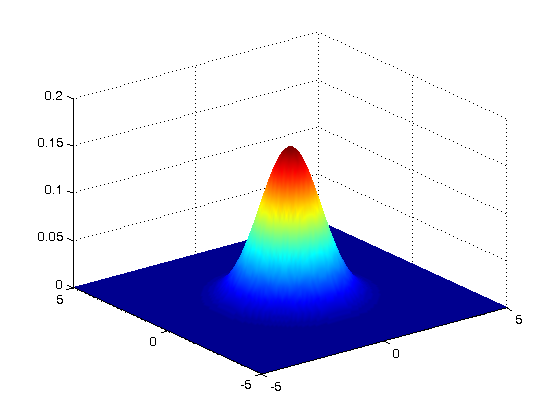
\includegraphics[scale=0.3]{gauss2d.png}
    \caption{2D Gaussian Function}
    \end{minipage}
    \begin{minipage}{0.5\textwidth}
    \centering
    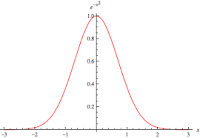
\includegraphics[scale=0.5]{gauss1d.png}
    \caption{1D Gaussian Function}
    \end{minipage}
\end{figure}

Gaussian functions  have two added advantages:
\begin{enumerate}
    \item $\phi$ is rapidly decreasing to 0 in all directions (i.e. the limit in any increasing direction away from $\vec{0}$ heads to 0 very rapidly)
    \item $\phi$ is smooth. In fact, $\phi$ is infinitely differntiable and all the derivatives are rapidly decreasing
\end{enumerate}
Functions such as $\phi$ are Schwartz functions and are extremely useful in approximating other functions because
of their desirable properties. 




Two important ways we can manipulate the Gaussian function are:
\begin{enumerate}
    \item we can move the center by a simple translation of the input from $\vec{x}$ to $\vec{x} - \vec{x}_0$
    \item we can change the spread by using a multiplier $\epsilon> 0$, i.e. $e^{-\epsilon \Vert x \Vert^2}$. 
    This multiplier has the effect of gathering the function around its center (larger values of $\epsilon$) or
    spreading the function out away from its center (smaller values of $\epsilon$).
\end{enumerate}

\begin{figure}[h]
    \centering
    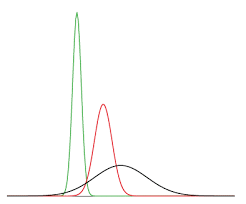
\includegraphics[scale=0.6]{gauss_diff.png}
    \caption{Different Gaussian Function}
\end{figure}

\section*{Interpolation using Radial Functions}
To use the radial functions in interpolation is fairly straightforward.
Suppose we are given a set of values in $\mathbb{R}^n$
\[
\vec{x}_1, \vec{x}_2, \dots, \vec{x}_n
\]
with accompanying real valued outputs
\[
y_1, y_2, \dots, y_n.    
\]
We can center a Gaussian radial function at each input by forming the functions
\[
\phi_k(\vec{x}) = e^{-\epsilon \Vert \vec{x} - \vec{x}_k \Vert^2}    \qquad \text{ for $1 \leq k \leq n$} 
\]
where we use $\epsilon > 0$ as a parameter that can be adjusted in the interpolation.

We then build the approximating function by summing the $\phi_k$'s as follows
\[
\phi(\vec{x}) = \sum_{k=1}^n c_k \phi(\vec{x}_k).
\]
Our goal  is to find values for $c_k$ that fit the given data values. 

By substituting the known data values into $\phi$ we obtain a system of $n$ equations
\[
y_1 = \phi(\vec{x}_1), \quad y_2 = \phi(\vec{x}_2), \dots, y_n \phi(\vec{x}_n).
\]
with each equation having the $n$ unknows $c_1, c_2, \dots, c_n$.
A linear system of $n$ equations with $n$ unknowns. 
Results from mathematics tell us that the system is solvable (that is, the associated matrix is invertable).
Therefore, we can find the missing values by standard means.

\section*{Properties and Results}
The resulting function $\phi$ gives a means to interpolate and extrapolate for values not in the given data set.
Because the function is the finite sum of infintely differentiable, rapidly decreasing functions, $\phi$ also 
enjoys the properties of being infinitely smooth and rapidly decreasing. The benefits of these properties
are somewhat dependent on the application. For instance, for reasonable values of $\epsilon$ the rapidly 
decreasing property will have have the following impact: Points further away from the given data values
used to create the function will tend to have approximates near zero. 
\end{document}
